% This is samplepaper.tex, a sample chapter demonstrating the
% LLNCS macro package for Springer Computer Science proceedings;
% Version 2.21 of 2022/01/12
%
\documentclass[runningheads]{llncs}
%
\usepackage[T1]{fontenc}
% T1 fonts will be used to generate the final print and online PDFs,
% so please use T1 fonts in your manuscript whenever possible.
% Other font encondings may result in incorrect characters.
%
\usepackage{graphicx}
% Used for displaying a sample figure. If possible, figure files should
% be included in EPS format.
%
% If you use the hyperref package, please uncomment the following two lines
% to display URLs in blue roman font according to Springer's eBook style:
%\usepackage{color}
%\renewcommand\UrlFont{\color{blue}\rmfamily}
%\urlstyle{rm}
%

\newcommand{\rdfexpression}[2]{%
	{\par\centering
		\begin{tabular}{@{}l l@{}}
			\texttt{#1} & \texttt{#2}
		\end{tabular}
		\par}%
}

\newenvironment{rdfexpressions}
{%
	\par
	\begingroup
	\centering
	\ttfamily
	\begin{tabular}{@{}r@{\ }l@{\ }l@{}l@{}}
	}
	{%
	\end{tabular}
	\par
	\endgroup
}

\begin{document}
%
\title{Bridging RiC-O and PREMIS: An Alignment Framework for Digital Archives}
%
%\titlerunning{Abbreviated paper title}
% If the paper title is too long for the running head, you can set
% an abbreviated paper title here
%
\author{Matthew Damigos\inst{1}\orcidID{0000-0003-0431-1482}\and 
Lina Bountouri\inst{1}\orcidID{0009-0006-1050-022X}\and 
Evangelia Thanou\inst{1}\and 
Eleftherios Kalogeros\inst{1}\orcidID{0000-0001-8080-6343}
}
%
\authorrunning{Thanou and }
% First names are abbreviated in the running head.
% If there are more than two authors, 'et al.' is used.
%
\institute{Laboratory of Digital Libraries and Electronic Publishing,\\ Department of Information Science, Ionian University, Corfu, Greece\\
\email{\{mgdamigos,alm.dimis2405,kalogero\}@ionio.gr}}
%
\maketitle              % typeset the header of the contribution
%
\begin{abstract}
	Digital archives require metadata models capable of representing both the archival context and the technical evidence necessary for their long-term preservation. RiC-O can be used to encode archival descriptions, while PREMIS provides detailed preservation metadata. These two models therefore address complementary dimensions of the same information environment. In this paper, we propose a lightweight bridge ontology that formalizes semantic relationships and class alignments between RiC-O and PREMIS, focusing on digital records and archives. The proposed framework combines class equivalence, specialization, and instance-level multi-typing without replacing PREMIS or refactoring RiC-O, preserving, in this way, the core semantics of both standards. 
%	In this way, it preserves the native semantics of both standards while enabling the construction of a unified, machine-readable knowledge graph that supports querying across archival descriptions and technical preservation metadata.
\keywords{RiC-O \and digital preservation \and PREMIS \and archival metadata.}
\end{abstract}
%
%
%
\section{Introduction}
Digital records have become the primary medium through which modern organizations, government institutions, and individuals document their activities, and preserve cultural memory (e.g., \cite{hawkins2022archives}).
%\cite{carroll2011comprehensive,liebermann2021born,jaillant2022can,hawkins2022archives,ries2022digital}. 
Unlike traditional paper-based archives, digital archives are not static physical repositories that hold fixed, human-readable documents. Instead, digital records exist as dynamic, software-dependent, and complex digital objects. The primary motivation for digital archives today extends far beyond simple long-term storage \cite{gattuso2017preservation}; it depends on technical and organizational conditions, such as file formats, software, hardware, storage environments, integrity checks, preservation actions, rights, and the evidence documenting those actions.
In this context, static, traditional metadata models do not suffice. Relational schemas and hierarchical, document-centric XML structures struggle to capture the highly interconnected nature of digital preservation environments. To ensure long-term authenticity, integrity, and intellectual accessibility across evolving technology stacks, digital archives require Linked Data models based on Semantic Web standards \cite{bizer2023linked}. 
%\cite{berners2023semantic,bizer2023linked}.


To capture the multidimensional nature of archival information, the archival community, through the International Council of Archives (ICA), developed Records in Contexts (RiC). RiC was developed to move archival description away from isolated hierarchical descriptions toward an entity-centric and relationship-oriented representation of records, agents, activities, events, functions, and other contextual entities~\cite{llanes2017records}. RiC - Conceptual Model (RiC-CM)~\cite{RICCM}
%~\cite{llanes2017records,RICCM} 
provides the conceptual model, while RiC-Ontology (RiC-O)~\cite{RiCO} expresses its concepts through RDF and OWL, making them suitable for Linked Data environments. This semantic orientation is particularly relevant to digital archives because information can be distributed across heterogeneous systems and benefit from explicit links between records, actions, people, software, policies, and evidence. Since RiC-O focus on modeling historical, organizational, and contextual provenance, it lacks explicit, fine-grained semantic constructs to model operational digital preservation microservices and technical object characteristics. 

On the other hand, the PREMIS Data Dictionary for Preservation Metadata~\cite{premis_data_dictionary_2015} is the widely-used international standard for documenting the preservation metadata of digital objects, including the operational lifecycle of digital objects, preservation events, rights, and technical dependencies. While PREMIS provides detailed technical granularity, it relies on external systems to supply the archival descriptions that give preserved objects their evidential meaning. 

When focusing on archives of digital records, the two models, RiC and PREMIS, consequently address complementary dimensions of the same information environment, where RiC emphasizes archival context, while PREMIS emphasizes preservation management. This constitutes the main problem addressed by this paper. In particular, this paper focuses on examining how to leverage the semantic expressiveness of Linked Data (specifically, RiC-O) alongside the operational preservation granularity of PREMIS to create a unified, machine-readable knowledge graph.  If archival description and preservation metadata remain isolated, a repository may know that a record exists and who created it, while storing preservation events and technical evidence elsewhere without a direct semantic bridge. Conversely, a preservation system may record a checksum, migration, or software dependency without representing the archival context that gives the preserved object evidential meaning.

To address this limitation, in this paper, we propose a lightweight bridge ontology that formalizes semantic relationships and class alignments between RiC-O and PREMIS v3, focusing on digital records and archives.  
Our approach provides a formal, machine-processable bridge without replacing PREMIS or refactoring RiC-O, also specifying  instance-level, multi-typing relationships between certain core structural entities. This approach preserves the native semantics of both domain standards, while enabling the implementation of a unified Knowledge Graph, allowing querying across archival descriptions and technical preservation metadata, as validated through concrete digital repository scenarios.
The rest of this paper is organized as follows: Section~\ref{sec:related-work} reviews the related work. Section~\ref{sec:preliminaries} provides the necessary formal background on OWL ontologies, RiC-CM/RiC-O, and PREMIS v3. 
Section~\ref{sec:alignment-framework} details the proposed extension and bridging architecture,
and Section~\ref{sec:conclusion} concludes the paper.
 with directions for future work. 


\section{Related Work}
\label{sec:related-work}


Recent research confirms that digital preservation increasingly depends on standardized metadata, provenance representation, and interoperability across heterogeneous information environments. Murillo and Yoon identify metadata, technological change, preservation strategies, and organizational issues among the recurring themes in contemporary digital-preservation literature \cite{murillo2021study}. Formenton and Gracioso emphasize the role of metadata standards in ensuring the persistence, intelligibility, access, and interoperability of archived Web resources, highlighting preservation metadata as an essential component of sustainable Web archiving \cite{formenton2022metadata}. From a provenance perspective, Bettivia et al. examine PREMIS alongside PROV and ProvONE, demonstrating that different provenance models address complementary preservation and workflow requirements rather than constituting interchangeable representations \cite{bettivia2022intersection}. Mosha and Ngulube similarly show, through a systematic review, that appropriate metadata standards are central to the continuous preservation, discovery, and reuse of research data \cite{mosha2023metadata}.  
These studies reinforce the need for preservation metadata,
providing the motivation for explicitly relating PREMIS preservation semantics to the archival context represented by RiC-O.


PREMIS has become a central framework for documenting the information required to preserve digital objects~\cite{woodyard2007implementing}. Implementation studies have nevertheless shown that PREMIS is normally adapted to the requirements and architecture of particular repositories, rather than deployed as a self-contained descriptive model \cite{donaldson2010implementing}. 
The PREMIS 3 ontology initiative revised this representation according to Linked Data principles and the PREMIS 3 Data Dictionary \cite{di2016premis,caron2018premis}. PREMIS has also been semantically combined with complementary models; notably, Li and Sugimoto integrate PREMIS and PROV-O to represent provenance of both digital resources and metadata \cite{li2014provenance}. These studies demonstrate the feasibility of ontology-based preservation integration, but do not address archival contextual description through RiC-O.

Records in Contexts addresses the complementary problem of representing archival resources through rich networks of records, agents, activities, events, and other contextual entities. RiC-O realizes this model in RDF/OWL and supports graph-oriented archival description. Practical work includes the RiC-O Converter, which transforms EAD and EAC-CPF descriptions into RiC-O RDF datasets \cite{clavaud2023ric}, and applications of RiC to scientific correspondence and historical legal archives \cite{santos2023applying,dimitriou2025describing}. Recent research also demonstrates that RiC can support extension and semantic alignment: Mikhaylova and Metilli extend RiC-O with the ITDT ontology for architectural archives \cite{mikhaylova2023extending}, while Bountouri et al. map RiC-CM to CIDOC-CRM to improve interoperability between archival and cultural-heritage models \cite{bountouri2023semantic}. Recent analyses additionally emphasize RiC's graph-based and contextual reconceptualization of archival description and provenance \cite{stephano2024recontextualization}.
%\cite{feliciati2021archives,stephano2024recontextualization}.


\section{Preliminaries}
\label{sec:preliminaries}
Ontologies provide formal vocabularies for representing concepts, properties, and relationships in a domain~\cite{gruber1993translation}. In other words, an ontology maps the basic concepts of a domain, defines the relationships between them, records their properties, and establishes the rules that govern them~\cite{antoniou_semantic_web_primer_2025}. Formally, an ontology O is defined as the tuple $O=<C, R, I>$, where C is the set of Classes / Concepts, R is the set of Relations / Properties, I is the set of Individuals / Instances of classes in C. 
To define ontologies in the Semantic Web context, RDF
%~\cite{w3c_rdf11_2014} 
represents information as subject-predicate-object triples, RDFS
%~\cite{w3c_rdfs_2014} 
supports classes and hierarchies, and OWL
%~\cite{w3c_owl2_2012} 
provides richer logical constructs for equivalence, specialization, restrictions, and reasoning~\cite{hendler2020semantic}. In the following, we use the RDF/RDFS properties
\texttt{rdfs:subClassOf} and \texttt{rdf:type} (or its abbreviation \texttt{a}) to define class specialization
and instance-level class membership, respectively, as well as the OWL
properties \texttt{owl:equivalentClass} and \texttt{owl:sameAs} to define
class-level semantic equivalence and instance-level identity, respectively.
To use multiple ontologies, one approach is to use a Bridge Ontology~\cite{kalfoglou2003ontology}, which acts as a decoupled semantic mediation layer that imports the necessary namespaces of the underlying ontologies and defines alignment rules without refactoring the underlying ontologies.


\subsection{Records in Context - Conceptual Model and Ontology}
The RiC-CM, developed by the International Council on Archives (ICA), seeks to integrate traditional archival description standards, such as ISAD (G), ISAAR (CPF), ISDF, and ISDIAH, within a unified conceptual framework~\cite{RICCM}. Unlike older hierarchical models, the RiC-CM is based on an entity-centric approach; archival information is organized around entities, attributes, and relationships, enabling data interlinking in Semantic Web and Linked Open Data environments~\cite{RICCM}.  

The basic entities of RiC-CM are the Record or Record Set, which corresponds to the archival record itself or a set of records (e.g., collections, fonds, series, folders). The Agent, is the person, organization, or group that creates, manages, or uses the records. Instantiations represent the physical or digital embodiments of Record Resources (the superclass of Record and Record Set). The Activity, which relates to activities or responsibilities and is directly linked to the creation of records and the Event, which includes actions and processes such as the creation, transfer, modification, or preservation of records. The model is complemented by entities such as Place and Date, which help to comprehensively capture the historical and functional context of the records. 

RiC-O~\cite{RiCO} is the OWL implementation of RiC-CM, providing a formal and machine-processable representation of its entities and relationships in RDF. 
Note that RiC-O~\cite{RiCO} is not a strict one-to-one translation of RiC-CM into OWL. While preserving the conceptual structure of RiC-CM, it introduces additional classes and properties required for an operational RDF/OWL representation, such as classes including \texttt{rico:Concept}, datatype properties for literal values, and object properties for linking entities. Moreover, some RiC-CM relations are represented in RiC-O both directly through object properties and, where richer description of the relation itself is required, through dedicated Relation classes.


\subsection{PREMIS (Preservation Metadata: Implementation Strategies)}


PREMIS is a well-known metadata standard designed to support the long-term management and preservation of digital objects~\cite{premis_data_dictionary_2015}. It focuses exclusively on the needs of digital preservation, prioritizing the authenticity, integrity, accessibility, and long-term usability of digital objects. PREMIS model is given in multiple representations/serializations, such as XML Schema (for traditional structured records)  and OWL / RDF ontologies (for Linked Data implementations)~\cite{caron2018premis}. The conceptual structure of PREMIS is based on four core entities: Object, Event, Agent, and Rights. 
%Figure~\ref{fig:premis} illustrates the classes of PREMIS 3 OWL ontology, as well as their subclass relations.
Notice that PREMIS ontology has been defined in terms of other well-established ontologies, such as PROV-O, FOAF and Dublin Core. PROV-O  is used to model provenance and execution history, while FOAF (Friend of a Friend)  is leveraged to represent human agents and organizations, and Dublin Core is mainly used to define Preservation Policies. It's worthy of note that PREMIS ontology is also extended through the Preservation Vocabulary\footnote{See \url{http://id.loc.gov/vocabulary/preservation}} provided by Library of Congress; e.g., the Event Type \texttt{creation} is defined as a subclass of the class \texttt{premis:Event}.

%\begin{figure}
%	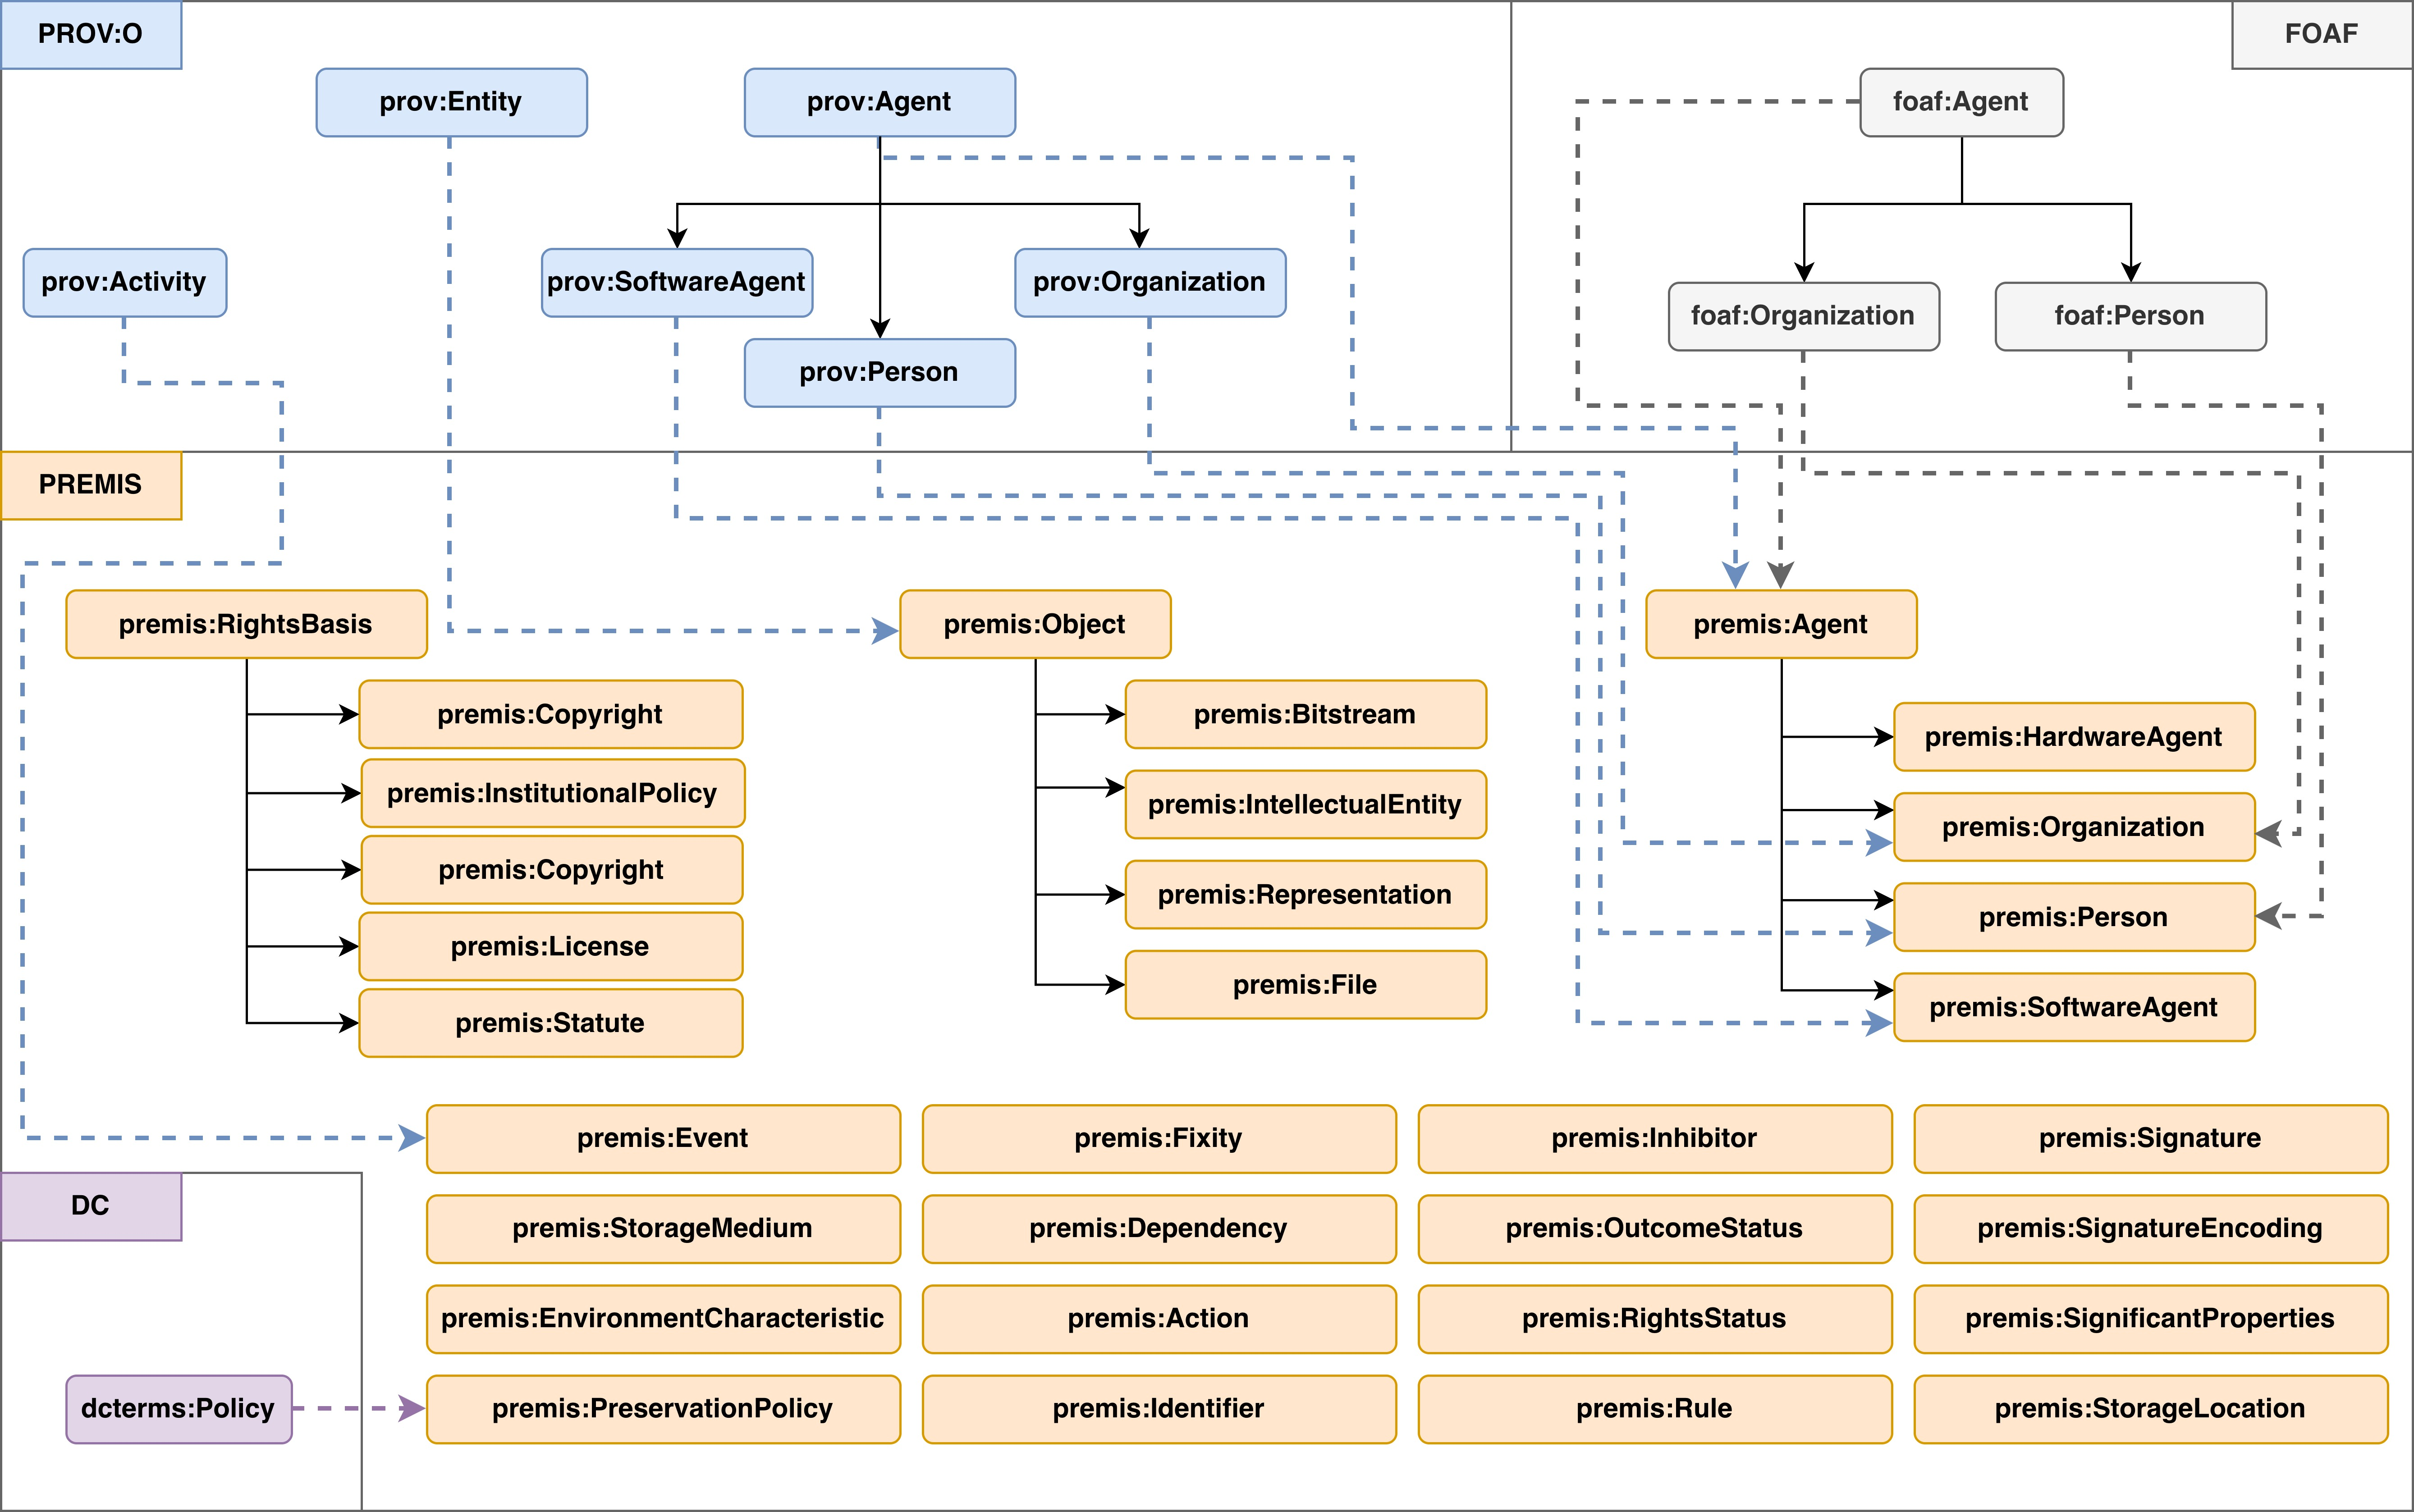
\includegraphics[width=\textwidth]{PREMIS-ontology.jpg}
%	\caption{Overview of PREMIS.} \label{fig:premis}
%\end{figure}





\section{Bridging RiC-O and PREMIS: Semantic Alignment Framework}
\label{sec:alignment-framework}


This section focuses on presenting the interoperability framework designed to bridge the RiC-O and PREMIS (v3) ontologies. Let us initially understand the context and need for such an alignment, by using a simple example. 
Consider a born-digital record issued on 2008-10-14, by the Ministry of Interior (\texttt{brg:Ministry\_Interior}) to document the administrative decision approving a municipal infrastructure funding allocation (\texttt{brg:Approve\_Funding}). The record is originally created in legacy Word format (\texttt{infra\_funding.doc}) and stored for long-term preservation. The document was later migrated to DOCX format (\texttt{infra\_funding.docx}), on 2024-09-10, to ensure compatibility with modern technology. A RiC-O metadata file captures the archival description, linking the record (\texttt{brg:Infra\_2008\_412}) to its creation date, creator, the approval activity it documents etc. Concurrently, PREMIS records operational preservation metadata, including file size, SHA-256 fixity fingerprints, and the automated format migration event (brg:Migration\_DOCX) executed by a software agent (brg:LibreOffice\_v7.5). 

To represent the aforementioned example through an RDF data graph, we depict a representative subset of this graph in Figure~\ref{fig:example}.
The white-colored nodes represent instances of RiC-O classes, the orange-colored nodes represent instances of PREMIS classes, and the dual-colored nodes
represent multi-typed entities, described later in this section. Through this example, we can easily see that  
bridging both ontologies is essential, because while RiC-O captures the description of the records and treats the migration log itself as a newly documented record (\texttt{migration\_logs}), PREMIS provides the detailed technical evidence of the migration, and only their alignment guarantees that the modern \texttt{.docx} file remains  authentic to its 2008 \texttt{.doc} origin.

\begin{figure}
	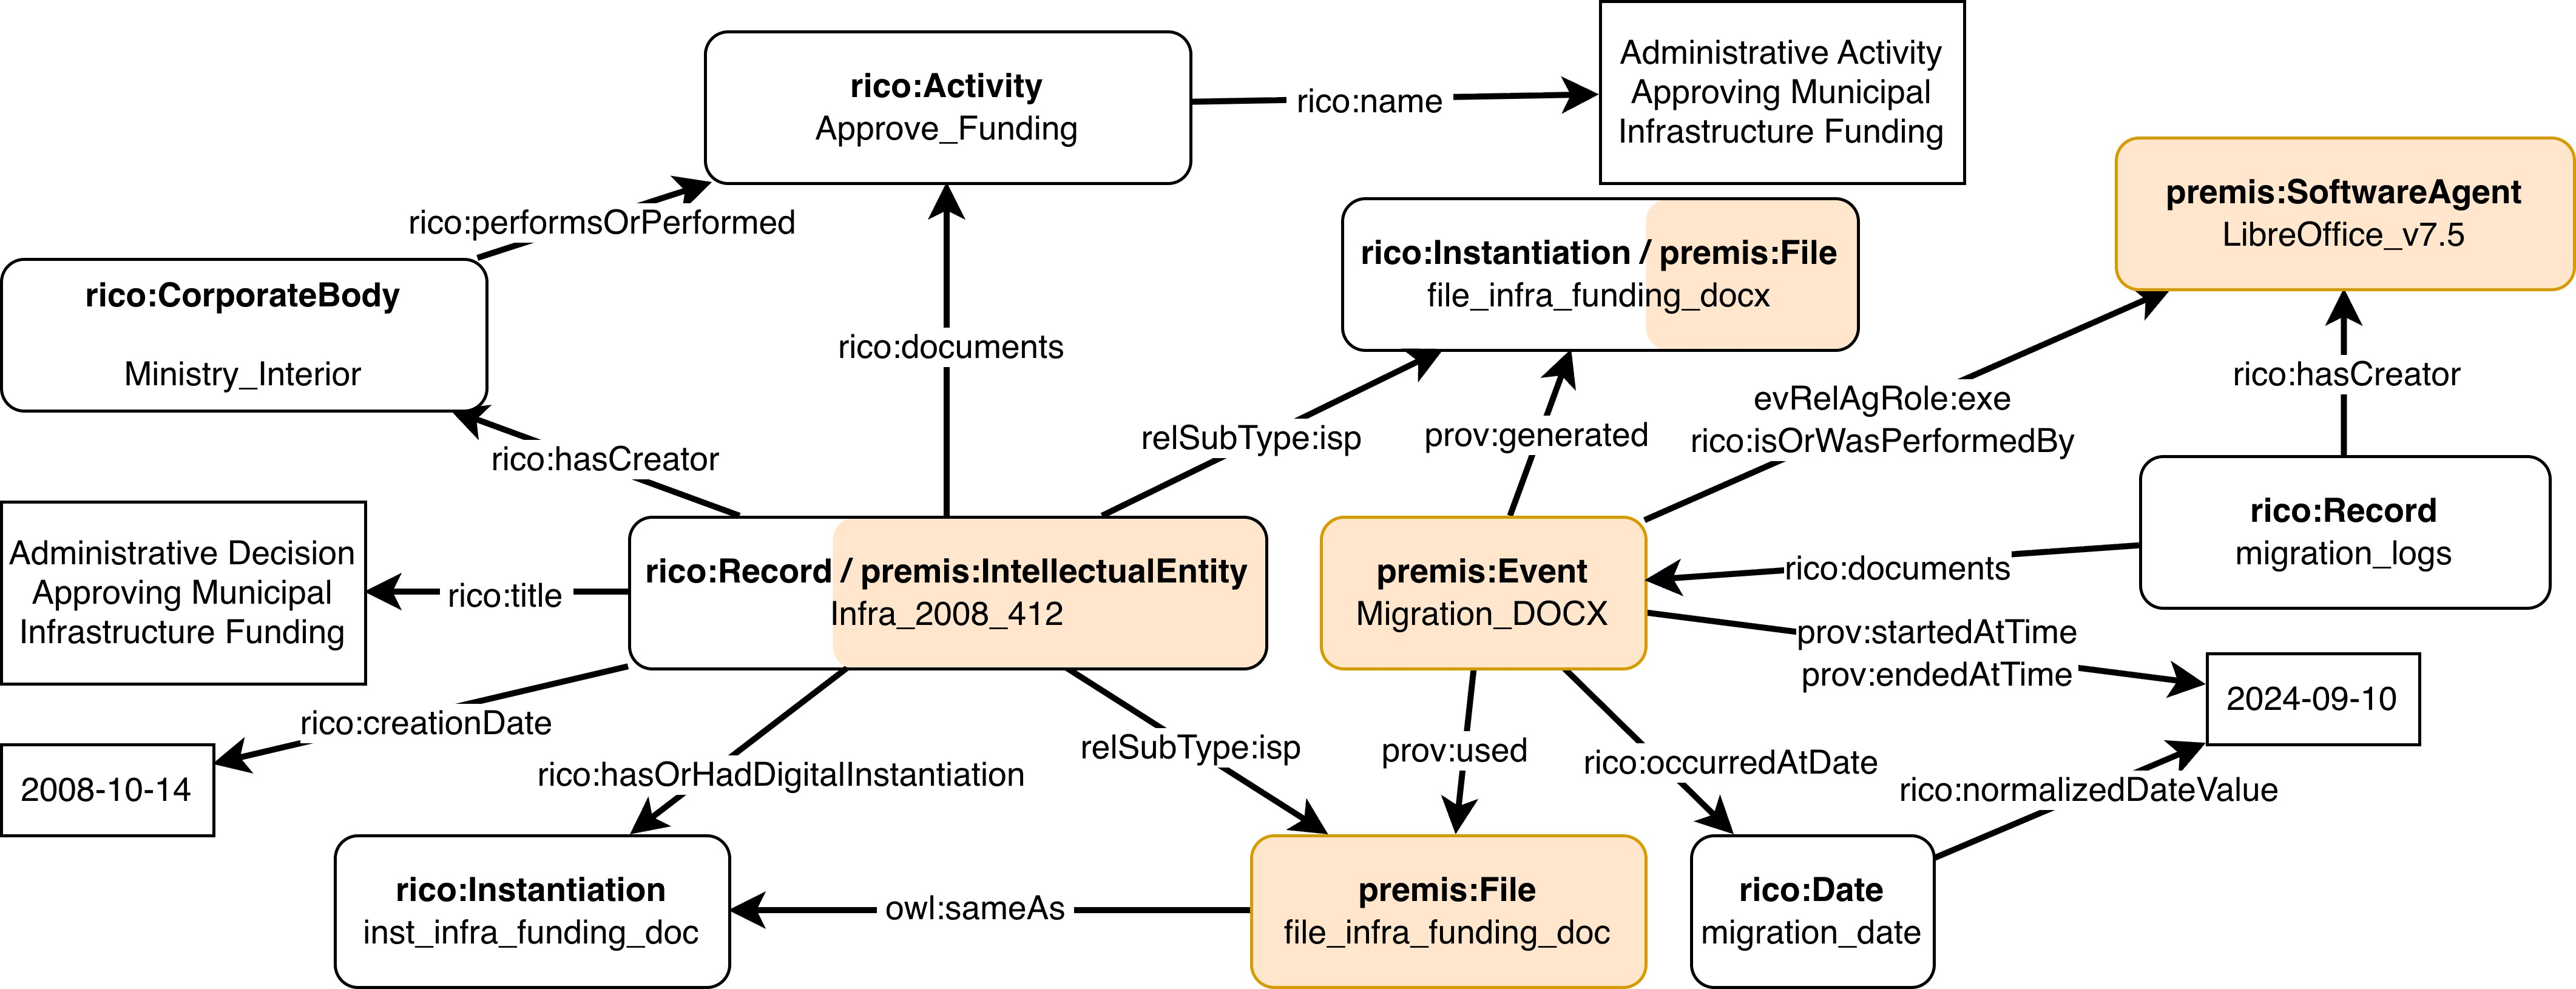
\includegraphics[width=\textwidth]{PREMIS-ontology-example.jpg}
	\caption{Example - PREMIS \& RiC-O.} \label{fig:example}
\end{figure}

To address this challenge, we focus on digital archives and records and present an alignment framework between RiC-O and PREMIS ontologies. One could think that such an alignment framework is given by directly modifying the source ontologies or asserting global class subsumptions across all core structural concepts. However, such an approach creates risks including ontological noise and unwanted inferential side effects (taking into account that PREMIS covers broader digital preservation domains beyond traditional archives), as well as compromises the maintainability of the unified model.
In this work, we handle semantic integration at the entity (class) level, leaving the exhaustive property alignment for future work. In particular, we propose a mapping of PREMIS classes to RiC-O ones and analyze its validity. Our alignment methodology relies on defining such a mapping through a lightweight, specialized Bridge Ontology.

 The proposed bridge is defined by focusing on how PREMIS classes are aligned with RiC-O entities (not aligning all the RiC-O classes with PREMIS ones). 
  The resulting framework focus on the context of digital records and archives and on relationships of three main categories: (1) \textit{Direct Class Equivalence} (\texttt{owl:equivalentClass}) where concepts share identical semantic boundaries, (2) \textit{Domain Specialization} (\texttt{rdfs:subClassOf}) where a PREMIS entity represents a specialized subset of a broader RiC-O concept, and (3) \textit{Instance-Level Multi-Typing} (\texttt{rdf:type}) for achieving entity reconciliation across structural instances via instance-level multi-typing.
  In instance multi-typing, individual real-world nodes in the RDF graph hold dual class assertions, satisfying both archival and preservation models simultaneously. Table~\ref{tab:rico-premis-mapping} summarizes the finalized semantic alignment across all core entities, while the analysis of the alignment is further discussed in the following section.
It's worthy of note that we also consider the OWL property \texttt{owl:sameAs} to specify instance-level equivalences, enabling the reconciliation of pre-existing, independent entities generated across distinct archival and preservation repositories. This approach ensures long-term extensibility as future iterations of PREMIS or RiC-O evolve.

	

\subsection{Detailed Entity Relationship Analysis}
\label{subsec:detailed-alignment}

In the previous section, we presented the main entities relationships defined in the proposed bridge ontology (see Table~\ref{tab:rico-premis-mapping}). In this section, we analyse how we end up with these relationships and why the remaining PREMIS classes are not associated with any RiC-O entity. As mentioned in the previous section, RiC-O and PREMIS are domain ontologies aiming to describe information of two overlapping domains. As a result, expecting that the full list of classes of each ontology can map to the classes of the other ontology would be unrealistic and, more importantly, semantically undesirable. RiC-O primarily models archival records, their provenance, context, agents, activities, rules, and instantiations, whereas PREMIS focuses on the operational requirements of digital preservation, including technical characteristics, preservation events, storage, dependencies, fixity, and preservation rights. Therefore, two ontologies intersect only where archival description and digital preservation refer to sufficiently compatible conceptual entities; e.g., both ontologies provide concepts for events, agents, identifiers, although they conceptualize these entities at different levels of abstraction.  


\emph{Preservation objects and archival things.} Initially, we focus on mapping the class \texttt{premis:Object}. In PREMIS, the class Object describes objects managed within preservation environments and processes. For example, such objects could be digital archives, such as a born-digital administrative decision, a digitized manuscript, or a preserved e-mail message, but also digital objects that do not constitute archival records, such as a software package, an emulation mechanism, or an auxiliary technical file maintained only to support preservation workflows. On the other hand, the class \texttt{rico:Thing} is defined as "any idea, material thing, or event within the realm of human experience"~\cite{RICCM}, which covers the objects defined using PREMIS, but not every instance of a \texttt{rico:Thing} is also a PREMIS object (e.g., instances of the classes Concept, Date or Place). Consequently, the bridge defines a subclass relationship, \texttt{premis:Object rdfs:subClassOf rico:Thing}, expressing that every PREMIS preservation object can also be interpreted as a RiC-O thing, while the inverse does not hold. This mapping therefore provides a general ontological anchor between the two models without implying semantic equivalence between their top-level concepts.

\begin{table}[ht]
	\begin{center}
		\scriptsize
		\begin{tabular}{l  l  c}
			\hline\hline
			\textbf{RiC-O Entity} & \textbf{PREMIS v3 Entity} & \textbf{Type of Relationship} \\
			\hline\hline
			\texttt{rico:Thing} & 	\texttt{premis:Object} & 	\texttt{rdfs:subClassOf} \\\hline
			\texttt{rico:RecordResource} & \texttt{premis:IntellectualEntity} & Instance-level Multi-typing\\
			&  & (\texttt{rdf:type}) \\
			\hline
			\texttt{rico:Instantiation} & \texttt{premis:Representation} & Instance-level Multi-typing\\
			&  & (\texttt{rdf:type}) \\\hline
			\texttt{rico:Instantiation} & \texttt{premis:File} & Instance-level Multi-typing\\
			&  & (\texttt{rdf:type}) \\\hline
			\texttt{rico:Activity} & \texttt{premis:Event} & \texttt{rdfs:subClassOf} \\\hline
			\texttt{rico:Identifier} & \texttt{premis:Identifier} & \texttt{owl:equivalentClass} \\\hline
			\texttt{rico:ActivityType} & \texttt{premis:Action} & \texttt{rdfs:subClassOf} \\\hline
			\texttt{rico:CarrierType} & \texttt{premis:StorageMedium} & \texttt{rdfs:subClassOf} \\\hline
			\texttt{rico:Agent} & \texttt{premis:Agent} & \texttt{rdfs:subClassOf} \\\hline
			\texttt{rico:Person} & \texttt{premis:Person} & \texttt{rdfs:subClassOf} \\\hline
			\texttt{rico:CorporateBody} & \texttt{premis:Organization} & \texttt{rdfs:subClassOf} \\\hline
			\texttt{rico:Mechanism} & \texttt{premis:SoftwareAgent} & \texttt{rdfs:subClassOf} \\\hline
			\texttt{rico:Mechanism} & \texttt{premis:HardwareAgent} & \texttt{rdfs:subClassOf} \\\hline
			\texttt{rico:Rule} & \texttt{premis:RightsBasis} & \texttt{rdfs:subClassOf} \\\hline
			\texttt{rico:Rule} & \texttt{premis:PreservationPolicy} & \texttt{rdfs:subClassOf} \\\hline
			\texttt{rico:Rule} & \texttt{premis:Rule} & \texttt{rdfs:subClassOf} \\\hline
			\texttt{rico:Mandate} & \texttt{premis:Statute} & \texttt{rdfs:subClassOf} \\\hline
			\hline
		\end{tabular}
	\end{center}
	\caption{Semantic Alignment between RiC-O and PREMIS.}
	\label{tab:rico-premis-mapping}
\end{table}

\emph{Intellectual entities and record resources.} An Intellectual Entity, in PREMIS, is typically defined as "a single intellectual unit for purposes of management and description"~\cite{premis_data_dictionary_2015} in a preservation environment; e.g., book, web page, map etc. Such an intellectual entity might be an archival record or a set of records (e.g., an archival file), including also record parts. Therefore, this is the  first entity that motivates an alignment between PREMIS and RiC-O. The RiC-O class that most closely corresponds to this entity is Record Resource, as it covers records, record sets, and record parts. However, a strict class-level assertion, in this case, is deliberately avoided between the PREMIS's Intellectual Entity and RiC-O's  Record Resource, since the semantic scope of the two classes does not fully coincide. For example, an Intellectual Entity may represent a preserved book, or software that is preserved, without necessarily be an archival record in the RiC-O sense. Conversely, when the Intellectual Entity corresponds to a resource that is described as part of a recordkeeping context (e.g., an administrative decision record, a migration log), the same individual can also be typed as a \texttt{rico:RecordResource}. Note that not all \texttt{rico:RecordResource} instances necessarily correspond to PREMIS Intellectual Entities, since some record resources may be described archivally without being managed as preservation-level intellectual units (e.g., a record part represented only for contextual description). Thus, we use an instance-level multi-typing rather than a global subclass relation, allowing only those PREMIS Intellectual Entities that genuinely function as archival record resources to receive both types. For the running example illustrated in Figure~\ref{fig:example}, the archival decision may be represented through the following triples, where the same resource is simultaneously the intellectual object managed for preservation and a record resource carrying archival provenance:
\begin{rdfexpressions}
	brg:Infra\_2008\_412 & a & premis:IntellectualEntity, & \\
	& & rico:RecordResource .
\end{rdfexpressions}

\emph{Representations, files and instantiations.}
The same approach applies to both 
PREMIS Representation and File, and RiC-O Instantiation.
A PREMIS representation represents a "digital or physical object instantiating or embodying an Intellectual Entity"~\cite{premis_data_dictionary_2015}, while the File entity models the "named and ordered sequence of bytes that is known to an operating system"~\cite{premis_data_dictionary_2015}; e.g., a record intellectual entity has a representation given by a sequence of TIFF images, where each image is modeled as an instance of the File class. In RiC-O, to express both representations of a record and a record part (typically, describes each page of the record), we use the Instantiation class, which represents "the inscription of information made by an agent on a carrier in any persistent, recoverable form as a means of communicating information through time and space"~\cite{RiCO,clavaud2021ica}. Similarly to Intellectual Entity and Record Resource, there are cases where a representation or a file instance defined using PREMIS is not an instantiation of a record resource (in essence, this is inherited by the corresponding intellectual entity), and cases where an instantiation instance is not managed within the preservation environment. Therefore, we also use an instance-level multi-typing approach to define instance of both PREMIS and RiC-O classes, according to the case. For example, in Figure~\ref{fig:example}, the instance \texttt{brg:file\_infra\_funding\_docx} of both the File and the Instantiation classes is defined as follows:
\begin{rdfexpressions}
	brg:file\_infra\_funding\_docx & a & premis:Representation,& \\
	& & rico:Instantiation .
\end{rdfexpressions}


\emph{Alignment of activities, actions and events.}
PREMIS events document actions (e.g., migration, validation, replication, and fixity checking) occurring during the lifecycle, and typically performed by an agent. Looking at RiC-O, the action class typically describes activity types. As a result, we consider it a subclass of the \texttt{rico:ActivityType} class. As for the instances of the PREMIS Event, they typically represent activities performed by Agents; hence, they also describe \texttt{rico:Activity} instances, since in RiC-O an "activity is specifically used to designate purposeful activity of an agent"~\cite{RICCM,RiCO}. One could argue that \texttt{premis:Event} is also a subclass of \texttt{rico:Event} to model events, such system failures. Although this type of events are semantically covered by \texttt{rico:Event} they are not modeled as instances of \texttt{premis:Event}. 
Continuing the example illustrated in Figure~\ref{fig:example}, the instance \texttt{brg:Migration\_DOCX} of the \texttt{premis:Event} (subclass of \texttt{rico:Activity}) uses the property \texttt{rico:occurredAtDate} to specify the date the migration process ran, and the property \texttt{rico:documents} to describe that the record \texttt{brg:migration\_logs} documents this event:
\begin{rdfexpressions}
	brg:Migration\_DOCX & a premis:Event ; & \\
	& rico:occurredAtDate brg:migration\_date . &\\	
	brg:migration\_logs & a rico:Record ; &\\
	& rico:documents brg:Migration\_DOCX . & \\
	brg:migration\_date & a rico:Date ; &\\
	& rico:normalizedDateValue "2024-09-10" . &
\end{rdfexpressions}
\emph{Alignment of agents.}
Another area where PREMIS and RiC-O considerably overlap is the representation
of agents. In PREMIS, an Agent includes as subclasses a person, organization, or software and hardware, which are involved in preservation activities,
%; for example, an archivist supervising a migration process, the archival institution responsible for the preservation of a record, or the software executing the migration.
RiC-O, on the other hand, provides the generic class \texttt{rico:Agent}, together with more specific classes for persons and corporate bodies. Consequently, the bridge
defines \texttt{premis:Agent} as a subclass of \texttt{rico:Agent},
\texttt{premis:Person} as a subclass of \texttt{rico:Person}, and
\texttt{premis:Organization} as a subclass of
\texttt{rico:CorporateBody}. The subclass relationship is preferred to class
equivalence since the PREMIS classes describe agents specifically in the
preservation context, while the corresponding RiC-O classes have a broader
archival scope. For example, the Ministry of Interior in our running example
may be described as a \texttt{rico:CorporateBody} because of its role in the
creation of the archival record, without necessarily participating as a PREMIS
preservation agent. Thus, an organization explicitly represented in
PREMIS as participating in a preservation process can also be interpreted as a
RiC-O corporate body.

PREMIS further distinguishes technical agents through the classes of software and hardware agents. Such
entities do not correspond to persons or corporate bodies in RiC-O; however,
they closely correspond to \texttt{rico:Mechanism}, which represents a
mechanism used by an agent in the performance of an activity. Consequently, both
PREMIS classes are defined as subclasses of \texttt{rico:Mechanism}. For
example, the software used to perform the migration in Figure~\ref{fig:example}
can be represented as: \texttt{brg:LibreOffice\_v7.5 a premis:SoftwareAgent}.
%
Through the bridge, the same instance is also inferred to be a
\texttt{rico:Mechanism}, thus allowing the preservation software to participate
in the archival description of the migration activity.

\emph{Storage media, carrier types and identifiers.}
The two ontologies also provide concepts for describing the medium in which
information is stored and the identifiers assigned to entities. RiC-O class \texttt{rico:CarrierType} covers all the storage mediums. Thus, we define \texttt{premis:StorageMedium} as its subclass. Furthermore, the class Identifier is defined in both ontologies and their semantics completely match; therefore, we define an equivalence relationship between them.


\emph{Rules, rights bases, and preservation policies.} Analyzing how both ontologies model the rules and mandates, we identify overlaps. In particular, PREMIS provides several classes for expressing the
normative context under which preservation actions are performed, including
Rights Basis, Preservation Policy, and Rule. In RiC-O, the broader class \texttt{rico:Rule} is used
to represent principles, regulations, policies, or other rules governing the
performance of activities. Therefore, the three PREMIS classes can be regarded as
preservation-specific kinds of RiC-O rules, and the bridge defines the subclass relationships as described in Table~\ref{tab:rico-premis-mapping}.
%
For example, a repository policy requiring records stored in obsolete formats
to be migrated to currently supported formats can be represented as a
\texttt{premis:PreservationPolicy}; through the bridge, the same policy is also
interpreted as a \texttt{rico:Rule} governing the corresponding preservation
activity. Similarly, the legal basis that permits a repository to reproduce or
migrate a digital record can be represented as a
\texttt{premis:RightsBasis} and, more generally, as a RiC-O rule.

A more specific correspondence exists for \texttt{premis:Statute}. A statute
represents a legislative basis under which preservation actions may be
authorized or restricted, while RiC-O provides the class
\texttt{rico:Mandate} for an authorization or requirement under which an agent
performs an activity. Consequently, the bridge defines
\texttt{premis:Statute rdfs:subClassOf rico:Mandate}. For example, a legal
deposit statute requiring an archival institution to preserve deposited digital
records may be represented as a PREMIS statute and, through the bridge, also as
a RiC-O mandate. Again, subclassing is preferred to equivalence because
\texttt{rico:Mandate} has a broader archival scope and is not restricted to
statutory preservation rights.

\emph{PREMIS classes without a RiC-O mapping.}
The remaining PREMIS classes are deliberately left without a corresponding
RiC-O class. This does not indicate that these concepts are irrelevant to
archival description, but rather that no RiC-O entity provides a sufficiently
close semantic counterpart to justify a class-level alignment. 


\section{Conclusion \& Future work}
\label{sec:conclusion}
This paper presented a lightweight semantic alignment framework between RiC-O and PREMIS v3 for digital archives. 
%The two ontologies address complementary aspects of the same information environment.
%Rather than modifying either source ontology, the proposed bridge defines selected class-level equivalence and specialization relationships and uses instance-level multi-typing where the semantic scopes of the corresponding classes do not fully coincide. 
This approach preserves the native semantics of both standards while enabling archival description and preservation metadata to coexist within a unified RDF graph.
%
The current work mainly addresses semantic integration at the entity level. Future work will focus on extending the bridge to a systematic alignment of RiC-O and PREMIS properties.
%, including preservation-event relationships, technical characteristics, rights, dependencies, and fixity information. 
Further work will also include the formal implementation and publication of the bridge ontology
%, validation through competency questions and reasoning, 
and evaluation on larger real-world digital archival datasets. Finally, the framework should be examined against future versions of RiC-O and PREMIS.
% in order to assess its maintainability and long-term extensibility.
% ---- Bibliography ----
%
% BibTeX users should specify bibliography style 'splncs04'.
% References will then be sorted and formatted in the correct style.
%
 \bibliographystyle{splncs04}
 \bibliography{bibliography}

\end{document}
